\section{Приклади}

\vspace{-\baselineskip}

\subsection{Одна з перших робіт з оцифровування дошки}

У 2004 році інженери з Microsoft Research \textit{Zhengyou Zhang}
та \textit{Li-wei He} представили свій алгоритм по скануванню написів
білої дошки.

В їхній роботі \cite{zhang:2004} обробляються фотографії білої дошки. Локалізується область
дошки, вирівнюється у прямокутну форму і бінаризуються написи без втрати
кольору.(рис. \ref{fig:zhang:2004}).
\begin{figure}[h]
  \centering
  \begin{subfigure}[b]{0.4\textwidth}
    \centering
    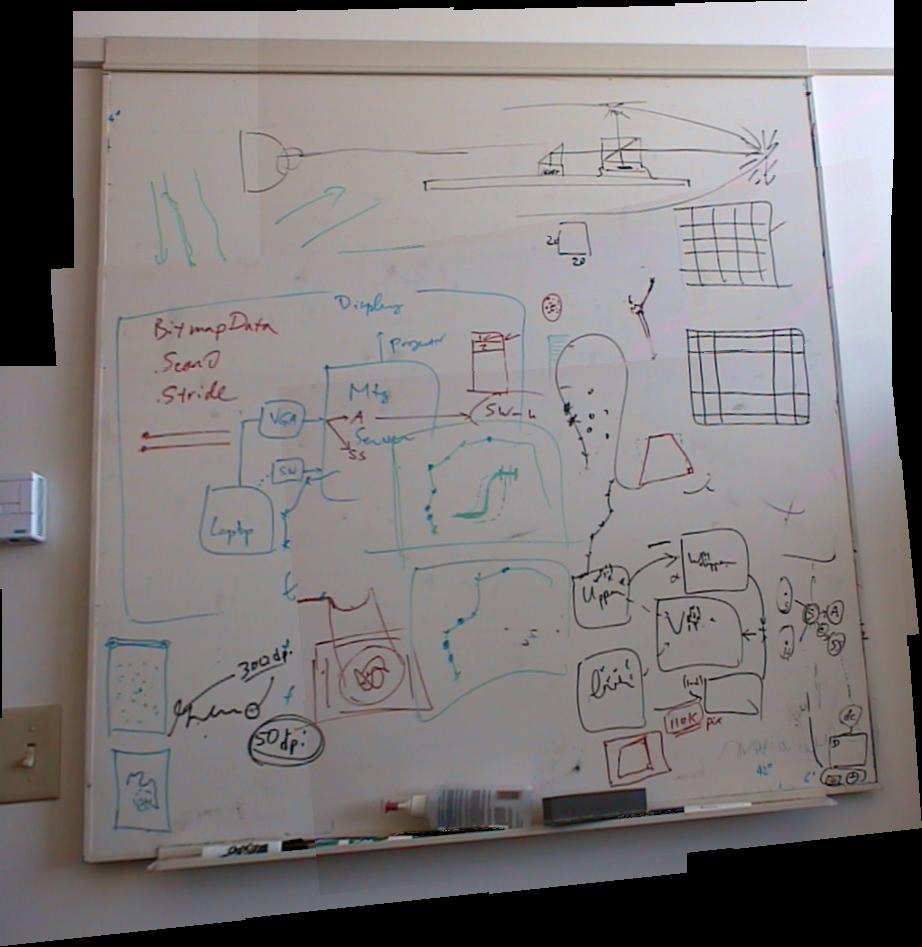
\includegraphics[width=\textwidth]{images/zhang_2004_1}
  \end{subfigure}
  \begin{subfigure}[b]{0.3\textwidth}
    \centering
    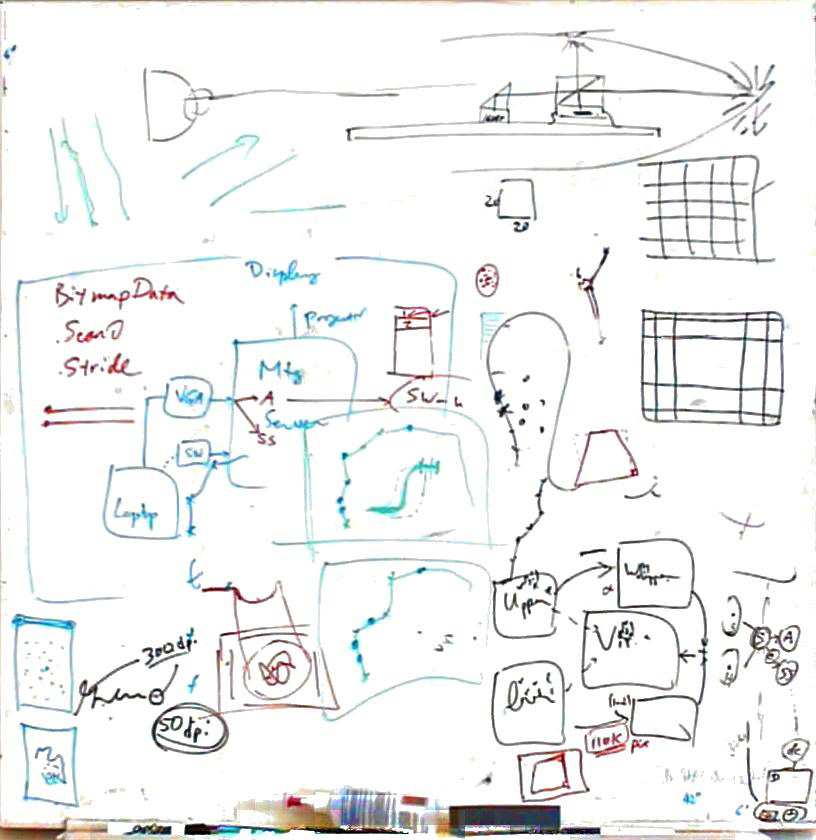
\includegraphics[width=\textwidth]{images/zhang_2004_2}
  \end{subfigure}
  \label{fig:zhang:2004}
  \caption{Демонстрація роботи алгоритму інженерів з Microsoft}
\end{figure}

Також автори реалізували склейку зображень дошки зроблених з різних
перспектив за допомогою гомографії. Гарна якість оцифрування дошки
досягається насамперед тим, що вона має білий колір, що в свою чергу
накладає обмеження для використання технології з дошками зеленого чи
чорного кольорів.
У наступній свої роботі \cite{zhang:2007} ціж самі автори побудували
систему, яка в реальному часі обробляє відеозапис, видаляє людину біля 
дошки за допомогою часової медіани, але в даному випадку немає 
панорамного склеювання знімків. Головна ідея роботи була зробити 
програму для телеконференсій.

\subsection{Автоматичне сканування дошки}

Автори даної роботи \cite{wienecke} створили програму яка переводить написи на білій 
дошці у цифрові. Вони реалізували локалізацію тексту та подальшу 
його обробку. Дана технологія не передбачає перекривання викладачем написів
або дошку іншого кольору відмінного від білого.

\begin{figure}[h]
  \centering
  \begin{subfigure}[b]{0.3\textwidth}
    \centering
    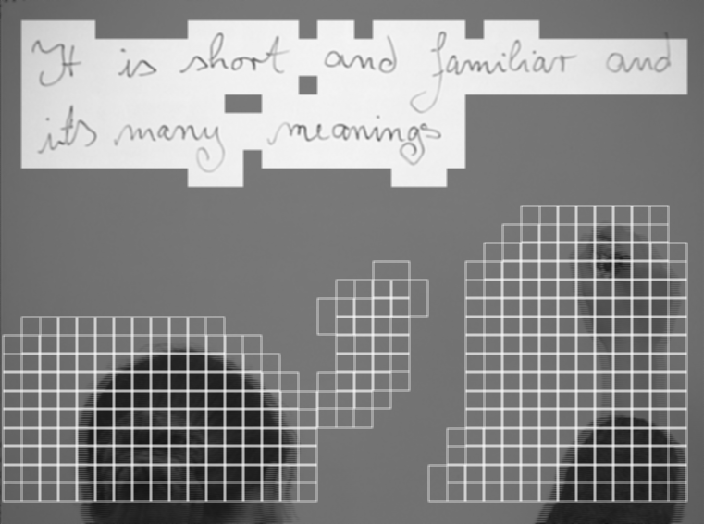
\includegraphics[width=\textwidth]{images/wienecke_1}
  \end{subfigure}
  \begin{subfigure}[b]{0.3\textwidth}
    \centering
    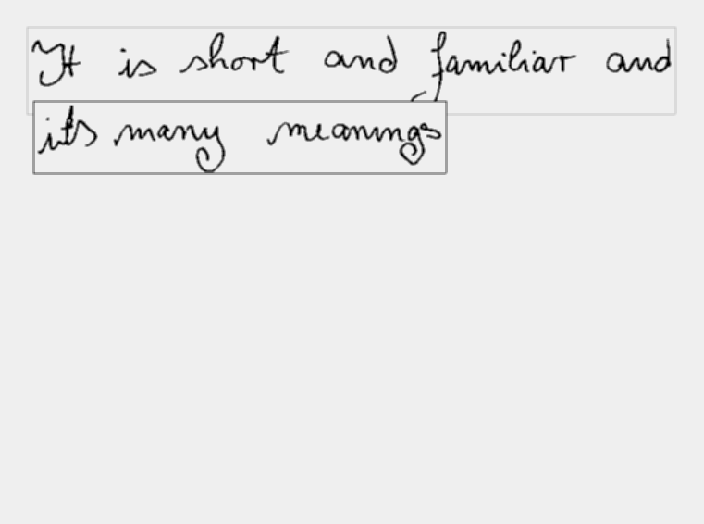
\includegraphics[width=\textwidth]{images/wienecke_2}
  \end{subfigure}
  \label{fig:wienecke}
  \caption{Демонстрація роботи сканування дошки}
\end{figure}

Можна помітити, що як і в попередній роботі гарна якість виокремлення написів
досягається тим що дошка білого кольору.

\subsection{Відстежування об'єкту та віднімання фону від Стенфорду}

У 2012 році науковці зі Стенфордського університету \textit{Alex Gonzalez, 
Bongsoo Suh, Eun Soo Choi} представили технологію \cite{sah} локалізацію дошки
(навіть такої яка розділена на частини), відстеження викладача та його
подальше прибирання. Алгоритм також може працювати з різними кольрами
дошок. Для прибирання викладача і всіх рухомих об'єктів автори також 
використали тимчасову медіану.

Дана програма не працює в реальному часі, оскільки всі операції над кадрами
відео займають тривалий час, не кажучи вже, що відео перед обробкою 
піддають компресії.

\begin{figure}[h]
  \centering
  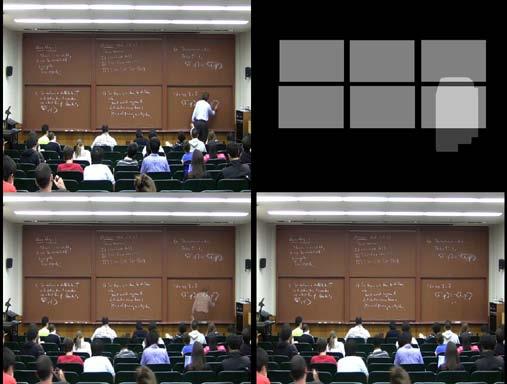
\includegraphics[width=0.5\textwidth]{images/sah}
  \caption{Приклад роботи авторів Стенфорду}
  \label{fig:sah}
\end{figure}

Головною особливістю даної роботи є те, що  алгоритм автоматично локалізує 
різну кількість дошок. Однак варто відмітити, що тестування відбувалось на
відеолекціях де камера знімає всю дошку і не рухається за викладачем. Тим більше
якість отриманих написів теж погана.

\subsection{Виокремлення написів дошки від Тайванського університету}

У 2014 році науковці із Тайванського університету представили свій аналог \cite{yeh} 
алгоритму по оцифровуванні дошки. Для видалення викладача автори застосували 
алгоритм кластеризації K-means. Для отримання бінаризованих написів з дошки 
використана адаптивне вирівнювання '(яке не ясно)'. Варто відмітити гарну
якість власного методу знешумлення.

\begin{figure}[h]
  \centering
  \begin{subfigure}[b]{0.3\textwidth}
    \centering
    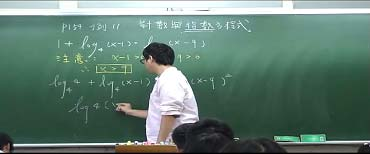
\includegraphics[width=\textwidth]{images/yeh_1}
  \end{subfigure}
  \begin{subfigure}[b]{0.3\textwidth}
    \centering
    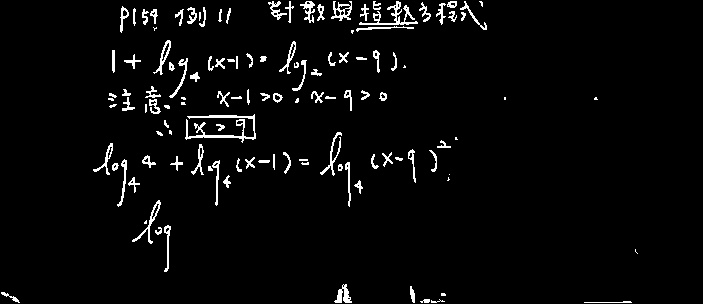
\includegraphics[width=\textwidth]{images/yeh_2}
  \end{subfigure}
  \label{fig:yeh}
  \caption{Демонстрація роботи сканування дошки}
\end{figure}

Автори не представили швидкість обробки всього відео. Щоб отримати якісну сегментацію
дошки та викладача потрібно, щоб кадр містив тільки викладача, причому щоб одяг викладача
був сильно відмінним від кольору дошки.

\subsection{Сучасна робота}

% На момент написання дисертації одними з новітніх робіт,
% де було використано модель Базельського університету,
% є методи відстеження обличчя \cite{Saito2016}
% та переносу виразу обличчя однієї людини іншій \cite{thies2016face}.
% Докладніше про них буде сказано в наступному підрозділі.
% Останньою відомою роботою
% є Large Scale 3D Morphable Models \cite{Booth:2017}~---~це
% генеративна модель обличчя, яка отримана з тривимірних знімків $10$ тисяч людей
% різної статі, віку та раси, що робить її дуже різноманітною та корисною
% (рис.~\ref{fig:problems:lsfm}).

% \begin{figure}[h]
%   \centering
%     \includegraphics[width=0.9\textwidth]{images/lsfm}
%   \caption{Приклади облич, що побудовані за допомогою LSFM}
%   \label{fig:problems:lsfm}
% \end{figure}
